%! Author = LucunJi
%! Date = 5/15/21

% Preamble
\documentclass[11pt]{article}
\usepackage[UTF8]{ctex}
% Packages
\usepackage{graphicx} % for figures
\usepackage{amsmath}  % for extended math markup
\usepackage{amssymb}
\usepackage{subcaption}
\usepackage{ulem}
\usepackage{hyperref}  % for url

\title{Uusi Aurinko 模组企划案\\
\ \\
\small{(该模组参加 2021 届 TeaCon Mod 开发大赛)}}
\author{\{LucunJi, XeKr, Neubulaeko\} $\in$ Team Ilmarinen}

% Document
\begin{document}
    \maketitle
    \begin{figure*}[ht!]
        \centering
        \includegraphics[width=.5\textwidth]{../Ilmarinen}

        \small{\textit{Ilmarinen}, the team name, comes from the immortal who can \textbf{Forge} and invent anything in Finnish mythology.}

        \small{队名\textit{伊尔玛利宁}取自于芬兰神话中能锻造与发明任何东西的不死者。}
        \label{fig:group}
    \end{figure*}

    \clearpage
    \tableofcontents

    \clearpage
    \section{简介}\label{sec:intro}
    Uusi Aurinko,芬兰语,即 New Sun,新太阳。它来自游戏 Noita 中的一系列成就任务:玩家收集太阳种子和五种元素,通过炼金术般的过程制造出新的太阳。

    通过将这一系列任务带入 Minecraft,Uusi Aurinko 模组添加了一些新的游戏后期玩法。
    玩家在拥有足够强大的装备后,再次游历一些远古遗迹,从宝箱中拾起曾经不敢接触的物品,通过一系列破坏性(甚至是毁灭性)的操作制造出一颗(或两颗)耀眼的(或黑暗的)太阳。

    为了保证原汁原味,游戏中的物品标注会使用 Noita 中的芬兰语命名和本地化的注释。

    \vspace{1em}
    这份企划案目前使用的图片大多为 Noita 游戏中的素材和截图,均来自 \href{https://noita.fandom.com/wiki/Noita_Wiki}{Noita Wiki}。
    为了规避版权问题,后续会换成自制素材。

    \clearpage
    \section{新增物品}\label{sec:new-items}

    \begin{figure}[ht]
        \centering
        \begin{subfigure}{3em}
            \centering
            \includegraphics[width=3em]{./imgs/Item_brimstone}
            \caption{}
            \label{fig:firestone}
        \end{subfigure}
        \begin{subfigure}{3em}
            \centering
            \includegraphics[width=3em]{./imgs/Item_waterstone}
            \caption{}
            \label{fig:waterstone}
        \end{subfigure}
        \begin{subfigure}{3em}
            \centering
            \includegraphics[width=3em]{./imgs/Item_thunderstone}
            \caption{}
            \label{fig:thunderstone}
        \end{subfigure}
        \begin{subfigure}{3em}
            \centering
            \includegraphics[width=3em]{./imgs/Item_stonestone}
            \caption{}
            \label{fig:stonestone}
        \end{subfigure}
        \begin{subfigure}{3em}
            \centering
            \includegraphics[width=3em]{./imgs/Item_kakke}
            \caption{}
            \label{fig:poopstone}
        \end{subfigure}
        \begin{subfigure}{3em}
            \centering
            \includegraphics[width=3em]{./imgs/Item_sunseed}
            \caption{}
            \label{fig:sunseed}
        \end{subfigure}
        \begin{subfigure}{3em}
            \centering
            \includegraphics[width=3em]{./imgs/Item_sunseed_2}
            \caption{}
            \label{fig:sunstone}
        \end{subfigure}
        \begin{subfigure}{3em}
            \centering
            \includegraphics[width=3em]{./imgs/Item_evil_eye}
            \caption{}
            \label{fig:evileye}
        \end{subfigure}
        \begin{subfigure}{3em}
            \centering
            \includegraphics[width=3em]{./imgs/Item_moon}
            \caption{}
            \label{fig:moon}
        \end{subfigure}
        \caption{来自 Noita 的物品}
    \end{figure}

    \subsection{元素石}\label{subsec:element-stone}
    Kiuaskivi(\ref{fig:firestone}):火石。
    烈焰人有极低概率掉落。地狱宝箱几率刷新。
    掉落物形式下不会被火焰摧毁。
    主手或副手持有时玩家获得火焰免疫(但是会有火焰效果),并随机在玩家周围生成火焰。

    Vuoksikivi(\ref{fig:waterstone}):水石。
    远古守卫者概率掉落,守卫者极低概率掉落。水中遗迹宝箱几率刷新。
    掉落物形式下不会被火焰摧毁。
    主手或副手持有时身上不会出现火焰效果。\\
    \sout{周围的岩浆源会变成黑曜石,流动的岩浆会变成圆石。(过于OP)}\\
    周围的岩浆源会变成一种类似浮冰的方块,随时间还原成岩浆源,流动的岩浆不受影响。\\
    \sout{身上所有非信标给予的效果,无论正面或负面,以双倍速度消退。(程序原}
    \sout{因无法实现)}\\
    在水中时获得水下呼吸效果。
    周围会受到水伤害的生物也会被缓慢地伤害。

    Ukkoskivi(\ref{fig:thunderstone}):电石。
    闪电苦力怕概率掉落。骷髅马概率掉落。末地宝箱几率刷新。
    掉落物形式下不会被火焰摧毁。
    持有时周围的水和金属块会随机出现扩散性的闪电特效。持有的玩家免疫闪电伤害。
    被电到的生物,除非持有电石,否则会受到伤害并获得缓慢效果。\sout{被电到的易燃物会燃烧。}

    Tannerkivi(\ref{fig:stonestone}):地石。
    基岩周围的石头被玩家挖掘时极低概率掉落。主世界的废弃矿坑、丛林神庙与沙漠神殿中的宝箱几率刷新。
    掉落物形式下不会被火焰摧毁。
    持有时周围的方块会随机变成泥土,容器方块以及液体、基岩、末地传送门框架、末地传送门等方块除外。
    玩家持有它近战攻击时造成小范围地震(周围方块变成对应的掉落沙\sout{,箱子等容器会被破坏})。

    Kakkakikkare(\ref{fig:poopstone}):粪石。
    僵尸极低概率掉落。主世界地牢宝箱概率刷新。
    掉落物形式下不会被火焰摧毁。
    玩家持有时随机造成自己短时间反胃,中毒。
    \sout{玩家周围的液体概率变成粪水(地狱中则会变成黑石)。(过于OP)}
    玩家周围的水变成粪水。玩家进入粪水也会获得反胃、中毒等 debuff。

    \subsection{太阳石}\label{subsec:solar-stone}
    Auringonsiemen(\ref{fig:sunseed}):太阳种子。
    击杀灵魂峡谷的特殊 boss 遗忘者 获得。
    掉落物形式下不会被爆炸或火焰摧毁。
    持有的玩家周围的沙子,沙砾,混凝土粉末等粉末物质随机消失并爆炸。
    \sout{给予玩家看到\textit{遗忘者}的能力。(多余)}

    Aurinkokivi(\ref{fig:sunstone}):太阳石。
    将\textit{太阳种子}在白天露天放置在沙漠神殿处获得。
    掉落物形式下不会被爆炸或火焰摧毁。
    第一次拾起后给予玩家凋零效果。
    周围粉末物质随机转化为火焰。\sout{给予玩家看到\textit{遗忘者}的能力。(多余)}
    在一秒内受到六次爆炸后变成一个最基础的\textit{新日}。

    \subsection{其他}\label{subsec:others}
    Paha Silmä(\ref{fig:evileye}):邪眼。
    八个恶魂眼泪围绕终末之眼合成,可以佩戴在头部。
    \sout{持有或}佩戴时给玩家看到\textit{遗忘者}的能力。
    生效时随时间减少耐久,不可附魔。

    Kuu(\ref{fig:moon}):微型月球。
    末地石和黑曜石合成。
    右键投掷出去后会在空中缓慢地漂浮。对着漂浮物右键可以将其收回背包。
    被投掷出去或持有时,将周围的\textit{新日}灵魂沙、弹射物和掉落物缓慢地拉向自己。自己也会因为这些实体而移动(相互吸引)。


    \clearpage
    \section{新增实体}\label{sec:new-entities}

    \subsection{遗忘之地怪物}\label{subsec:forgottens}
    \begin{figure}[ht]
        \begin{subfigure}{10em}
            \centering
            \includegraphics[width=10em]{./imgs/Monster_Boss_Ghost}
            \caption{Unohdettu}
        \end{subfigure}
        \begin{subfigure}{10em}
            \centering
            \includegraphics[width=10em]{./imgs/Monster_hpcrystal}
            \caption{Elvytyskristalli}
        \end{subfigure}
        \begin{subfigure}{10em}
            \centering
            \includegraphics[width=10em]{./imgs/Monster_snowcrystal}
            \caption{Haamukivi}
        \end{subfigure}\label{fig:entities}
    \end{figure}
    Unohdettu:遗忘者。
    这是一只白色,比恶魂略大,独眼,骷髅状的飞行生物。血量与凋灵相当。
    生成在灵魂峡谷中的特殊结构\textit{遗忘之地}中。
    除非借助邪眼、太阳石、太阳种子,玩家无法看见它。

    只会受到来源为玩家的伤害。无法看见它的玩家无法对它造成任何伤害。
    会被\textit{恢复水晶}治疗。攻击方式是朝玩家发射蓝色的激光。
    被击杀后固定掉落一个\textit{太阳种子}。

    Elvytyskristalli:恢复水晶。
    末地水晶的绿色版。破碎后不会产生爆炸,但是有较高的血量(100)。
    与\textit{遗忘者}一起在\textit{遗忘之地}中生成,一般会有4~6个。
    每隔一段时间尝试给附近的遗忘者恢复生命。
    破碎后掉落较多的恶魂之泪。

    Haamukivi:幽灵水晶。
    末地水晶的灰色版。破碎后不会产生爆炸,但是有较高的血量(100)。
    每隔一段时间检测周围的\textit{幽灵怪物}数量。若被它生成的\textit{幽灵怪物}小于一定数量则补充生成一些。
    破碎后所有被它生成的\textit{幽灵怪物}会一起消失。掉落较多的恶魂之泪。

    幽灵怪物:
    灰色、半透明版的原版怪物。他们被\textit{幽灵水晶}生成。
    它们不会受到任何伤害,但是在距离生成它们的\textit{幽灵水晶}过远时会消失。生成它们的\textit{幽灵水晶}消失时,它们也会消失。
    以下怪物有幽灵版本:
    \begin{itemize}
        \item 僵尸
        \item 尸壳
        \item 僵尸村民
        \item 骷髅
        \item 流浪者
        \item 蜘蛛
    \end{itemize}

    \subsection{新日}\label{subsec:new-sun}
    \begin{figure}[ht]
        \includegraphics[width=\textwidth]{./imgs/New_Sun}
        \caption{Uusi Aurinko}\label{fig:new-sun}
    \end{figure}
    Uusi Aurinko:新日。
    随机将周围末地传送门以外的\textbf{任何}方块变成流动的岩浆(不是岩浆源)。
    内部会有一些不会被摧毁的发光方块提供亮度。
    会朝着附近手中或漂浮中的\textit{微型月球}移动。
    周围的所有实体都会被持续地点燃,受到燃烧上海并被拉向它的中心。所有死亡的生物脚下都会生成流动的岩浆。

    \textbf{阶段一:}刚被创建时,最开始很小且较暗。在周围死亡100只生物后会变白、变亮并显著变大,进入二阶段。

    \textbf{阶段二:}接下来,玩家可以向内部投入元素石。投入的元素石会消失并使新日略微变大一些。此外:
    \begin{itemize}
        \item \textit{水石}使它颜色变紫。
        \item \textit{地石}使它变绿并增强引力效应。
        \item \textit{火石}使它变红并增强火焰伤害。
        \item \textit{雷石}使它变蓝并在周围随机生成闪电与爆炸。
    \end{itemize}

    \textbf{阶段三:}
    投入除\textit{粪石}以外的所有四种元素石后,它会显著变大并完成生长(阶段三)。

    如果在投入三种元素石后投入\textit{粪石},它会以一种“特别”的方式完成生长:
    体积几乎变为普通阶段三新日的两倍,颜色变成黑色,火焰伤害和引力效果变得极大。

    无论是否变成黑色,这一阶段的太阳如果在末地中,会朝着末地的$(0, 200, 0)$坐标缓慢移动;如果在主世界,则会朝着主世界的$(0, 200, 0)$坐标移动。
    当然,它依然会最优先选择朝着附近手中或漂浮的\textit{微型月球}移动。

    \textbf{湮灭:}
    完整尺寸的普通新日与黑色新日相遇时,二者会在剧烈的爆炸中湮灭。
    所有世界中的所有生物并获得强烈的燃烧、凋零与缓慢效果。玩家则会直接死亡,死亡信息是“xxx死于强烈的高速粒子射流”。

    \clearpage
    \section{新增进度}\label{sec:achievements}
    \begin{itemize}
        \item \textbf{掌中炽焱} \quad 条件:获得\textit{火石}
        \item \textbf{固态水。等等,这不是冰?!} \quad 条件:获得\textit{水石}
        \item \textbf{ElectroBOOM} \quad 条件:获得\textit{电石}
        \item \textbf{大地在颤动} \quad 条件:获得\textit{地石}
        \item \textbf{呕——} \quad 条件:获得\textit{粪石}
        \item \textbf{追忆} \quad 条件:击杀\textit{遗忘者}
        \item \textbf{转变} \quad 条件:造出\textit{新日}
        \item \textbf{血与火的成长} \quad 条件:\textit{新日}周围死亡100个生物
        \item \textbf{太阳照常升起} \quad 条件:成长完全的普通\textit{新日}移动到主世界的$(0, 200, 0)$附近
        \item \textbf{腐坏} \quad 条件:\textit{新日}变成黑色
        \item \textbf{新秩序} \quad 条件:成长完全的黑色\textit{新日}移动到末地的$(0, 200, 0)$附近
        \item \textbf{毁灭性中和} \quad 条件:黑色与普通\textit{新日}相互碰撞
    \end{itemize}


    \clearpage
    \section{美术设计}\label{sec:artistic}

    模组的整体美术风格应该尽量贴近 1.16.5 的原版像素风格。物品设计极为简单,暂且不表。一些复杂的问题请见下文。

    \subsection{新日}\label{subsec:design-sun}

    新日在设计时需要给予玩家足够的体积感和压迫感。具体体现在大小对比、环境氛围和粒子效果。严格来说,粒子效果也可以算作环境氛围的一部分。
    可以用这几张截图(\ref{fig:sun-screenshots})感受一下 Noita 中新日与玩家(旁边紫袍法师)的大小对比和氛围感。

    新日的巨大体积感是最重要的。目前考虑过以下几种模型:
    \begin{itemize}
        \item \sout{直接做成一个球体,对渲染技术的要求较高。}
                \sout{例子是是龙之研究 mod 的能量塔与反应堆(\ref{fig:sphere-de})。}
        \item \sout{做成多个正方体组成的球体。为了较好地实现球体效果,}
                \sout{ 模型和贴图会很复杂。}
        \item 做成正方体或接近正方体的形状。模型和贴图都会比较简单。
        \item \sout{做成单个永远用正面朝着玩家的平面贴图。非常简易。例子是 Minecraft 的火焰弹、雪球。}
    \end{itemize}
    模型可能还会加上旋转的动态效果。

    环境氛围则可以通过让玩家靠近时屏幕颜色变红来营造炽热感。
    考虑到运行压力,粒子效果可能会削减得较少。
    作为粒子效果的替代,玩家靠近时,屏幕可以贴上一张动态半透明的图片(类似南瓜头的遮罩效果)来模拟热浪和粒子迸发效果。
    这里提到的屏幕贴图替代粒子效果,可以参考游戏《超时空方舟》中雪地关卡的“迎面暴雪”效果(\ref{fig:chronoark-snow})。
    “雪花”近大远小,近快远慢,且在近处有眼睛没有对焦的模糊效果。

%    ----------------- 图片 -----------------
    \begin{figure}[ht]
        \begin{subfigure}{18em}
            \centering
            \includegraphics[width=18em]{./imgs/Sun_small}
            \caption{阶段一,尺寸并不大。区区金黄色的发光球体而已,似乎可以简单地操控}
        \end{subfigure}
        \begin{subfigure}{18em}
            \centering
            \includegraphics[width=18em]{./imgs/Sun_medium}
            \caption{阶段二,新日已经吞噬了100个生物。此时已经能感受到体积感}
        \end{subfigure}
        \begin{subfigure}{18em}
            \centering
            \includegraphics[width=18em]{./imgs/Sun_full}
            \caption{阶段三,新日很大并且放射出大量光芒和粒子}
        \end{subfigure}
        \begin{subfigure}{18em}
            \centering
            \includegraphics[width=18em]{./imgs/Sun_dark}
            \caption{阶段三(黑色),巨大的压迫感}
        \end{subfigure}
        \caption{来自视频《\href{https://www.bilibili.com/video/BV1CZ4y1w7AL}{【Noita彩蛋】啦啦啦~种太阳☀}》的几张截图}
        \label{fig:sun-screenshots}
    \end{figure}

    \begin{figure}[ht]
        \centering
        \includegraphics[width=\textwidth]{./imgs/Draconic_Evolution_sphere}
        \caption{《龙之进化》的球体。
        来自视频《\href{https://www.bilibili.com/video/BV11541187n8}{【我的世界模组教程】龙研最稳定比例的反应堆}》}
        \label{fig:sphere-de}
    \end{figure}

    \begin{figure}[ht]
        \centering
        \begin{subfigure}{\textwidth}
            \centering
            \includegraphics[width=\textwidth]{./imgs/ChronoArk_snow_1}
            \caption{}
        \end{subfigure}
        \begin{subfigure}{\textwidth}
            \centering
            \includegraphics[width=\textwidth]{./imgs/ChronoArk_snow_2}
            \caption{}
        \end{subfigure}
        \caption{《超时空方舟》中的“暴雪迎面”效果。
        来自视频《\href{https://www.bilibili.com/video/BV1K5411r7cd}{ChronoArk推倒死神(游戏已经汉化啦)}》}
        \label{fig:chronoark-snow}
    \end{figure}
%    ----------------- 图片完 -----------------


    \clearpage
    \subsection{装饰方块}\label{subsec:decorative-blocks}
    为了展示模组,也需要制作一些装饰性的方块。由于我(禄存)不擅长材质和贴图这方面的事情,这里只能给出一个大致的思路。

    展馆呈四棱锥形,类似玛雅金字塔,外部设有四条通往顶部的台阶。顶部有一块仪式用的平顶。
    展馆内部镂空,竖有几根支撑用的柱子和几个较矮的底座。模组的物品就放在展馆内部的底座上。

    展馆主要的建筑材质是土黄色的石砖(\ref{fig:texture-screenshots}),硬度和黑曜石相当。一些地方还有金黄色的字符。
    放置物品的底座上面还有亮绿色的字符(\ref{fig:pedestals})。
    可以用 Minecraft 中的“标准银河字母”来达到 Noita 中字符相似的效果。当上面的物品被移走时,底座上的字符会变成红色。

    \begin{figure}[ht]
        \begin{subfigure}{0.5\textwidth}
            \centering
            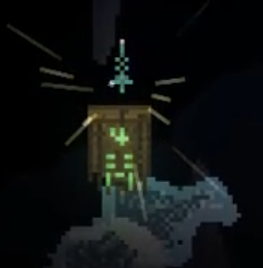
\includegraphics[width=16em]{./imgs/Wand_pedestal}
            \caption{}
        \end{subfigure}
        \begin{subfigure}{0.5\textwidth}
            \centering
            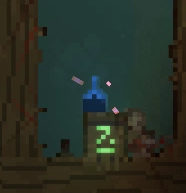
\includegraphics[width=16em]{./imgs/Potion_pedestal}
            \caption{}
        \end{subfigure}
        \caption{两种 Noita 中的底座}
        \label{fig:pedestals}
    \end{figure}

    \begin{figure}[ht]
        \begin{subfigure}{\textwidth}
            \centering
            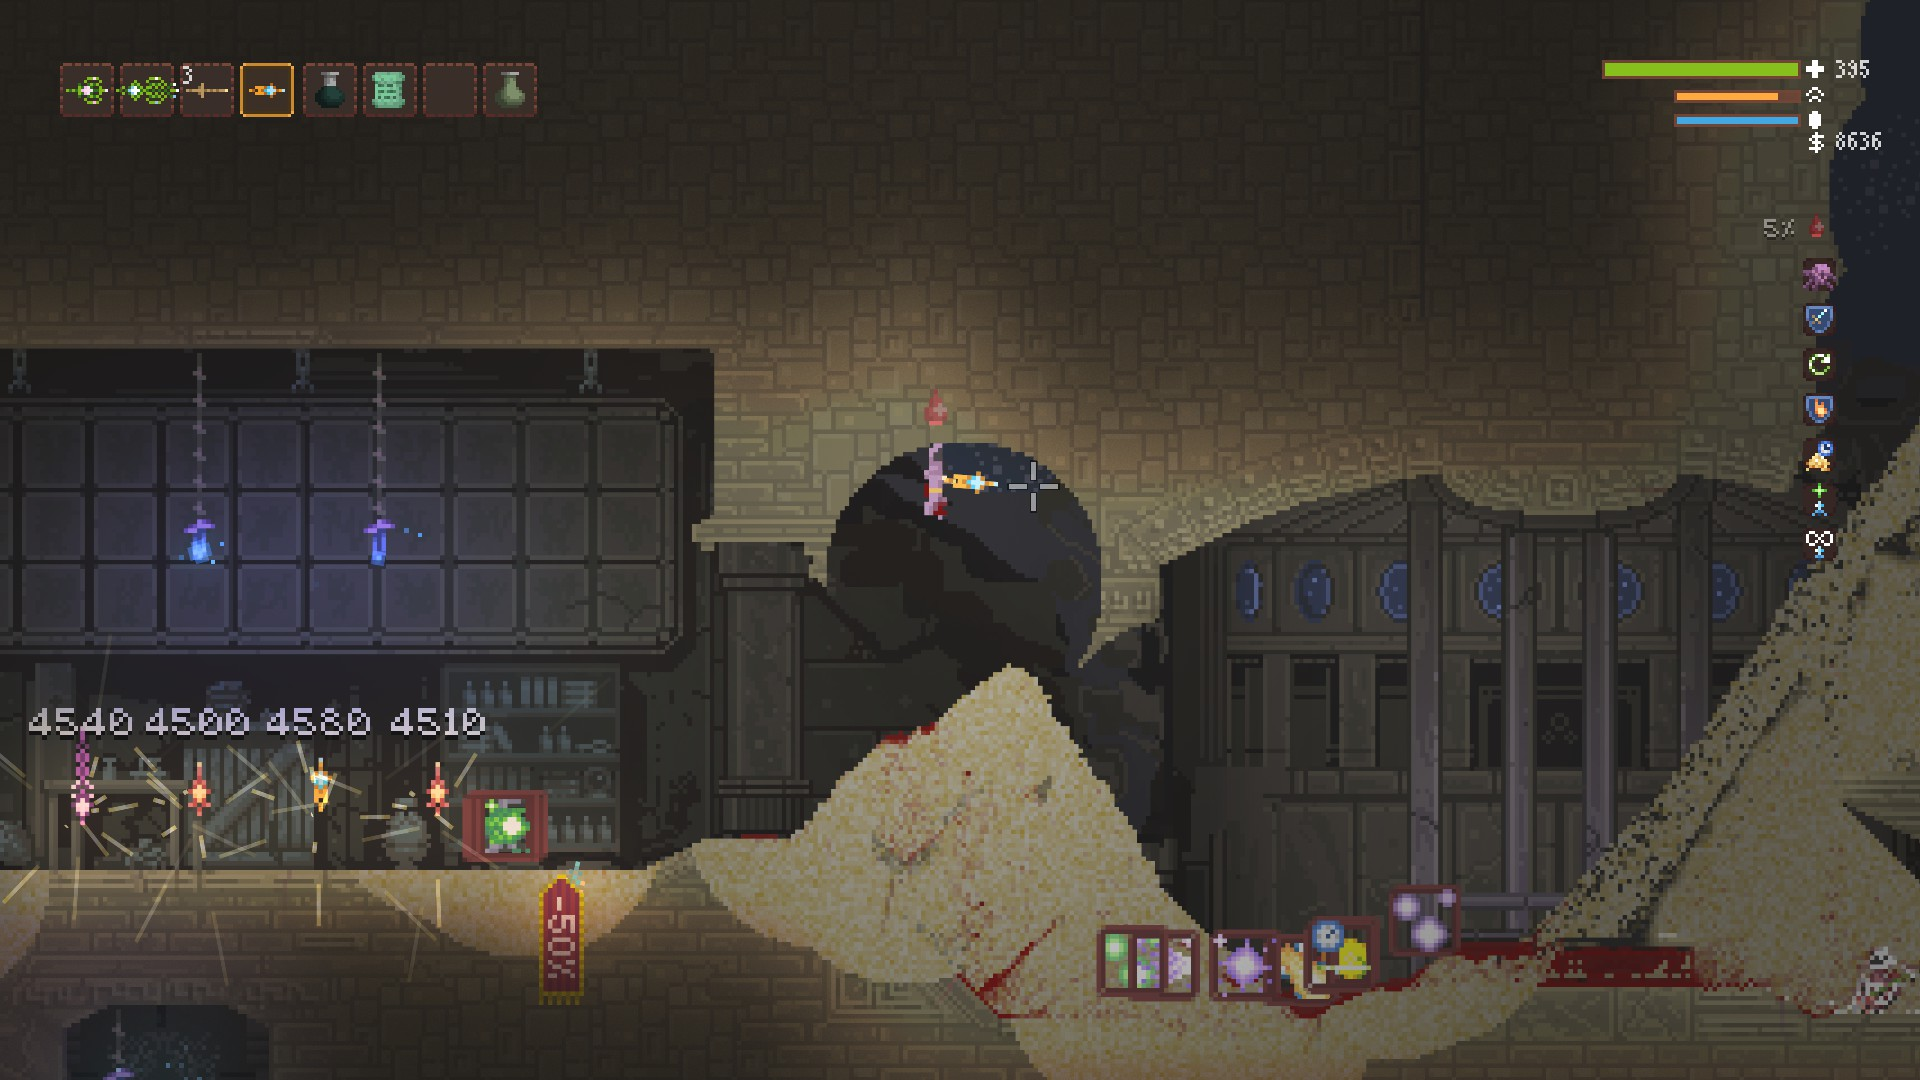
\includegraphics[width=\textwidth]{./imgs/20210622001701_1}
            \caption{}
        \end{subfigure}
        \begin{subfigure}{\textwidth}
            \centering
            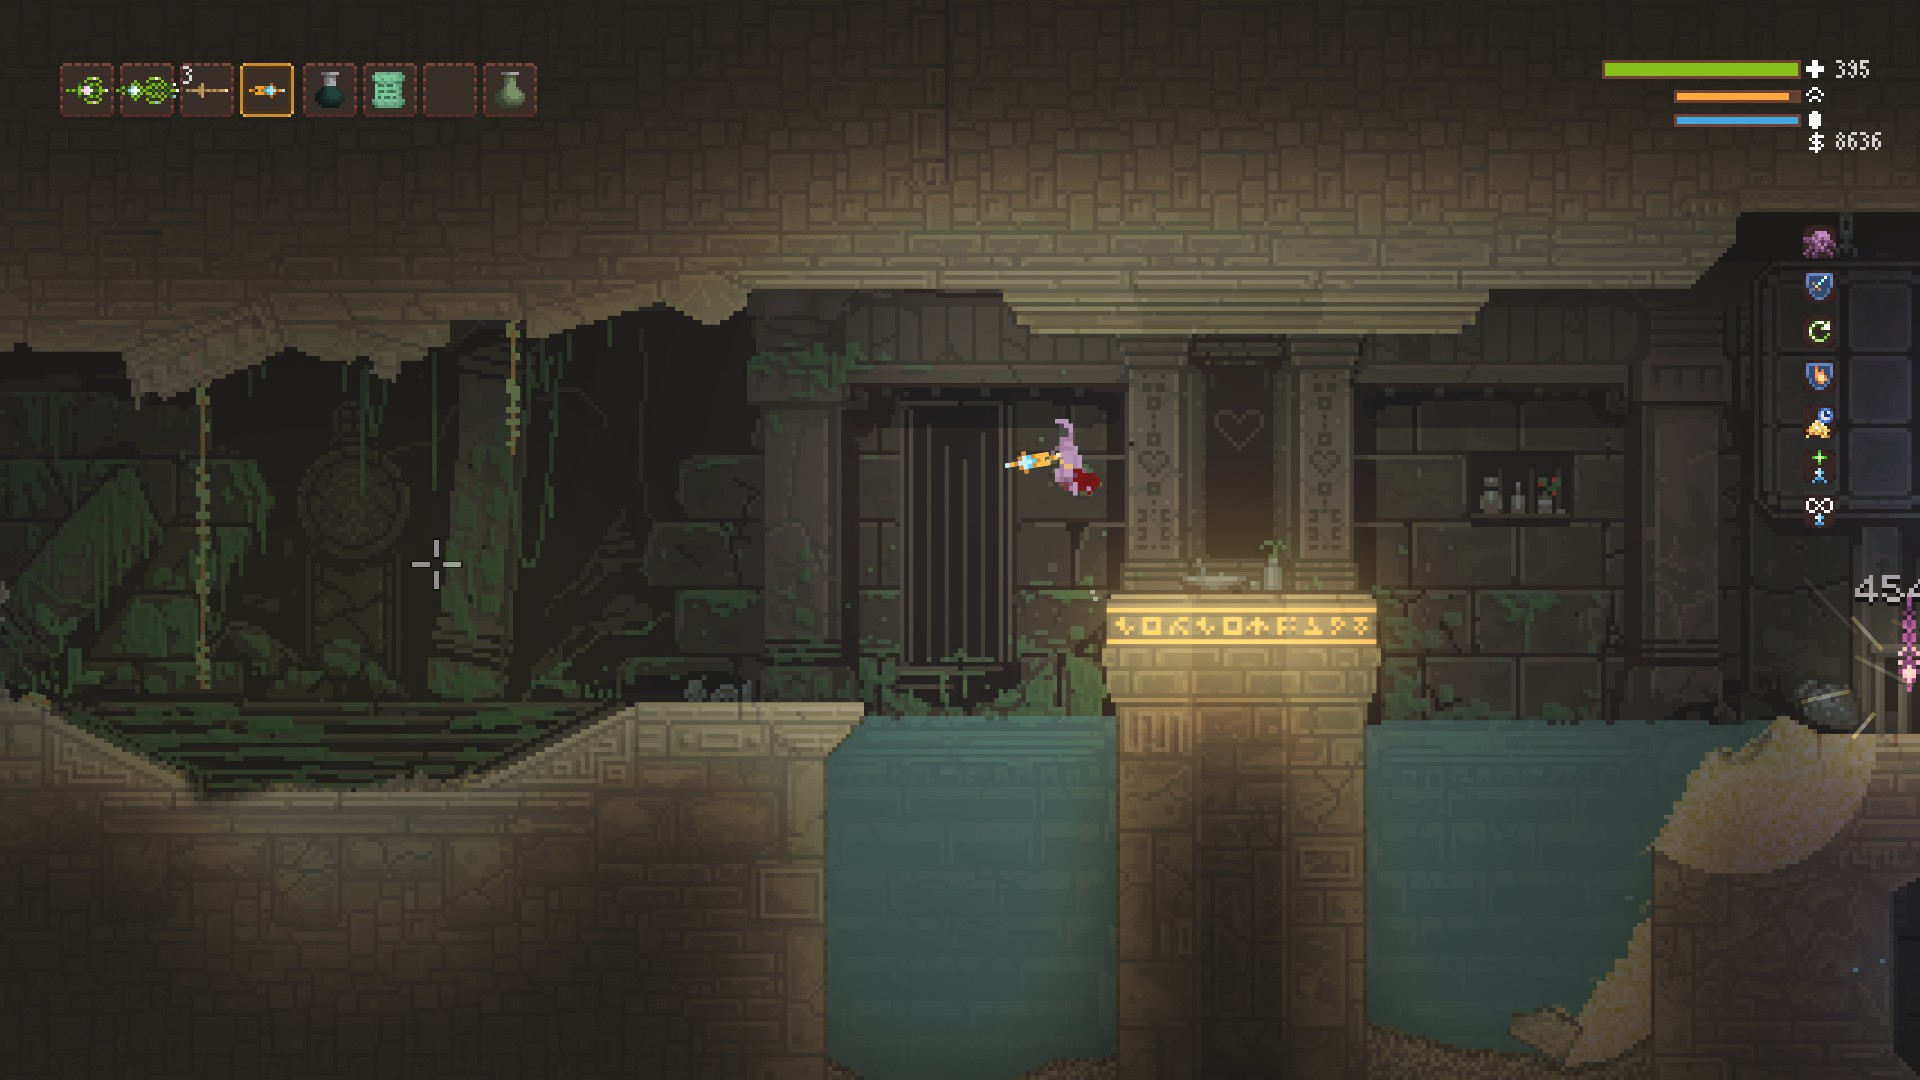
\includegraphics[width=\textwidth]{./imgs/20210622001712_1}
            \caption{}
        \end{subfigure}
        \caption{一些游戏内的截图,展示了材质大致的概念}
        \label{fig:texture-screenshots}
    \end{figure}

\end{document}